\documentclass[class=book, crop=false, oneside]{standalone}
\usepackage[subpreambles=true]{standalone}

\usepackage{../../style}

\graphicspath{{./assets/images/}}
% arara: pdflatex: { synctex: yes, shell: yes }
% arara: latexmk: { clean: partial }
\begin{document}
\chapter{Introduzione}

\section{Cos'è un compilatore}
Il compilatore, generalizzando, è un meccanismo che trasforma il codice sorgente in codice eseguibile.
Nota però che il codice eseguibile è machine dependent, difatti noi studieremo i principi generali di questa traduzione ma dobbiamo tenere a mente il fatto che ogni tipo di macchina ha il suo linguaggio macchina che deve essere utilizzato per scrivere gli eseguibili da essa utilizzabili.


Se osserviamo il compilatore gcc diciamo subito che è in sviluppo da 20 anni e consta di ben più di due milioni di righe di codice! Il gcc però è un ottimo esempio di compilatore, quindi in realtà è un po’ fuori dalle righe.


L’esempio classico di utilizzo di un compilatore è la traduzione da codice c in assembly.
Un codice in assembly, tuttavia non è ancora eseguibile. Manca il passaggio di conversione da assembly a codice binario; tuttavia, questo passaggio non è così complesso dato che assembly ha una corrispondenza quasi 1:1 con il binario.
Ma quest’ultima traduzione non è l’unico passaggio mancante: rimane ancora da affrontare la fase di linking.

\section{Le fasi del processo di compilazione}
In questa sezione presentiamo le fasi del processo di compilazione come se fossero in pipeline, ma sappi che per ragioni di efficienza vengono spesso sovrapposte. Due punti fondamentali di questo processo sono i seguenti:
\begin{enumerate}
    \item Se scriviamo il programma in un certo linguaggio, lo dovremo compilare con il compilatore dedicato esattamente a quel linguaggio
    \item Quando scrivo codice per un certo compilatore devo rispettare la grammatica del linguaggio per cui il compilatore lavora
\end{enumerate}
La grammatica di un linguaggio definisce la struttura legale delle varie operazioni possibili in quel linguaggio; ad esempio, può definire questa forma per un’operazione di assegnamento:

\texttt{Identifier Assign Expression Semicolon}

Dove Identifier è un segnaposto per un qualsiasi identificatore (stringa) che può essere utilizzato dal programmatore.
Osserviamo quindi che in primis abbiamo questi due elementi: codice sorgente e grammatica.

Ora che abbiamo definito il punto di partenza, possiamo procedere con una descrizione delle fasi della compilazione.

\paragraph{Analisi lessicale}
Il primo passaggio che compie il compilatore è l’analisi lessicale.

Traduce un flusso di caratteri in un flusso di \emph{tokens}, ciò significa che risolve ogni “stringa” riconoscendo il suo ruolo. Per esempio, traduce:

\texttt{Pippo = 2*3}\\
In:

\texttt{<ID, pippo> ASS <NUM,2 > MUL <NUM,3> SEMCOL}\\
In questa fase i token che otteniamo contengono le informazioni sul tipo di dato o comando che ogni singola stringa identifica. “Si tratta di capire chi è chi”.

Nota che non vengono perse informazioni, non si tratta di una traduzione in cui la stringa dell’ID viene eliminata: si tiene la stringa “pippo” e vi si assegna il ruolo di identificatore (ID).

\paragraph{Analisi sintattica}
Dopo l’analisi lessicale arriva l’analisi sintattica.

Questa analisi verifica se la sequenza di token è aderente alla grammatica del linguaggio che stiamo utilizzando. Questa è la temuta fase in cui compaiono i syntax error.

Se rispettiamo le regole della grammatica il flusso di token viene tradotto in un parse tree (o meglio ancora, dipende dal compilatore, in un albero di sintassi astratta).\\
L’albero di sintassi astratta (abstract syntax tree, AST) è ottenuto dal parse tree compattando delle parti che non saranno utili nelle fasi seguenti della compilazione.

Ecco il parse tree che si può ricavare dal nostro esempio: 
\begin{figure}[H]
	\centering
	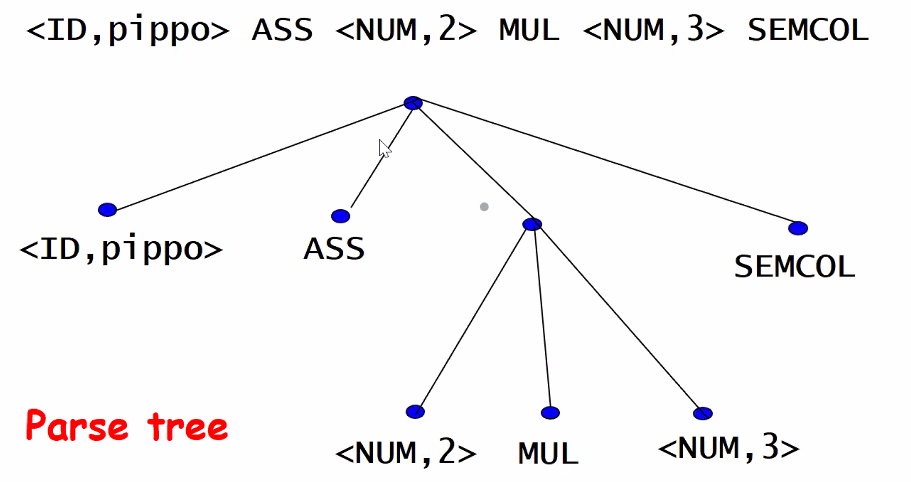
\includegraphics[width=0.9\textwidth,keepaspectratio]{parse_tree}
	\caption{Esempio di parse tree}
\end{figure}
La struttura del parse tree è derivata dalla grammatica del linguaggio. Ad esempio, \texttt{<NUM,2> MUL <NUM,3>} sono sottoalberi di \texttt{ASS} poiché la grammatica del linguaggio prevede che l’assegnazione abbia questa forma.
Più la struttura del parse tree è minimale più le fasi successive sono efficienti.

È qui che entra in gioco l’AST, che semplifica ancora lo schema:
\begin{figure}[H]
	\centering
	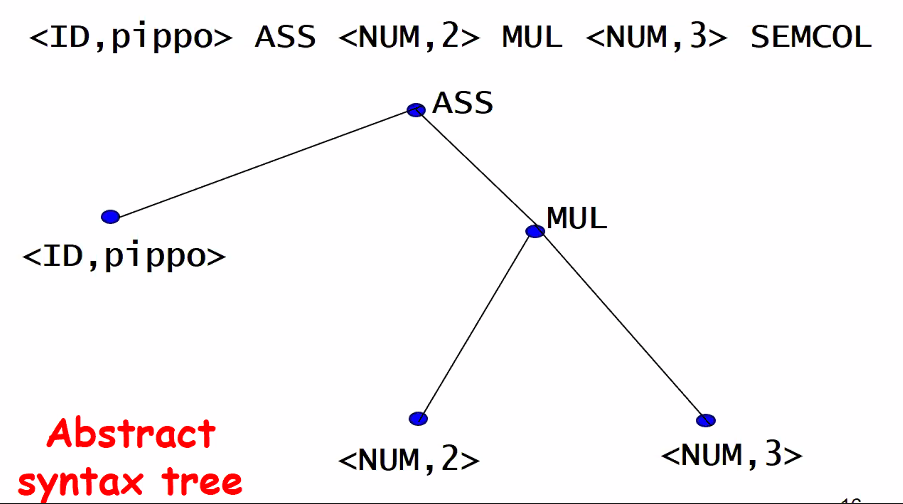
\includegraphics[width=0.9\textwidth,keepaspectratio]{abstract_syntax_tree}
	\caption{Esempio di abstract syntax tree}
\end{figure}
Il guadagno in complessità in questo caso è poco (abbiamo risparmiato tipo 3 nodi), ma in casi più complessi il risparmio è molto molto impattante.

Non è facile scrivere una grammatica che possa essere analizzata con efficienza da un compilatore e che generi parse tree più semplici possibili; vedremo in futuro.

È da notare che esistono svariate forme di compilatori, noi ne stiamo vedendo una presentazione generale, ma, in molti casi, fasi come creazione di parse tree e AST vengono spesso sovrapposte.

Nota importante:\\
L’output dell’analisi sintattica è chiamato \emph{tree}, ma non necessariamente è un albero: spesso può essere un grafo. Ad esempio in un’operazione del tipo:
\texttt{pippo = pippo * 2}
Il nodo pippo sarebbe collegato sia alla radice che all’operatore \texttt{ASS}, creando quindi un grafo.
%TODO: insrire immagine dell'AST dell'operazione pippo = pippo * 2

\paragraph{Analisi semantica}
Ora è la fase dell’analisi semantica.

Un esempio di operazione di analisi semantica è quello di capire se stiamo utilizzando il giusto operatore di moltiplicazione per l’operazione che vogliamo effettuare. Stiamo chiaramente riferendoci a quei linguaggi in cui esistono diversi significati per uno stesso operatore, come nel caso in cui l'operatore \texttt{MUL} può significare moltiplicazione sia tra interi sia tra float.

Quindi si può dire che in questo caso l’analisi semantica chiarisce quale significato ha l’operatore \texttt{MUL}: nell’esempio riportato sopra \texttt{MUL} = moltiplicazione tra due variabili di tipo \texttt{NUM}.
\begin{figure}[H]
	\centering
	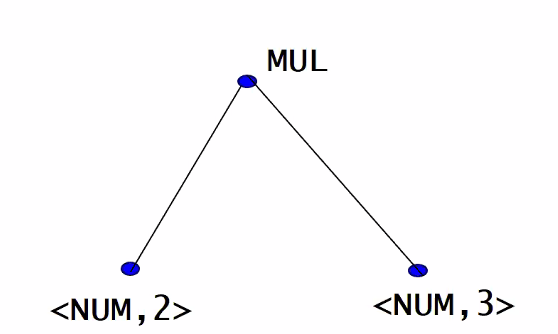
\includegraphics[width=0.7\textwidth,keepaspectratio]{semantic_analysis}
	\caption{La semantica di \texttt{MUL} deve essere specificata}
\end{figure}

\paragraph{Generazione del codice intermedio}
È il momento della generazione del codice intermedio.

In questa fase viene creato un codice testuale creato traducendo il parse tree. Queste istruzioni sono leggibili dall’uomo ma non è né assembly né codice effettivo, d’altronde si chiama intermedio, no?

Nel caso in figura sulla destra abbiamo il parse tree e sulla sinistra abbiamo un esempio del codice intermedio generato.
\begin{figure}[H]
	\centering
	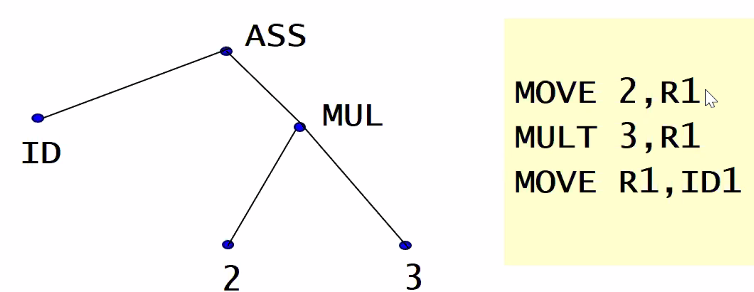
\includegraphics[width=0.9\textwidth,keepaspectratio]{codice_intermedio}
	\caption{Generazione del codice intermedio}
\end{figure}

\paragraph{Generazione del target code}
Questa fase consiste nella traduzione del codice intermedio nell’assembly della specifica macchina.

Il codice binario non è necessariamente il target code della compilazione. Ad esempio, potremmo essere su una VM e quindi generare una sorta di bytecode, o magari potremmo avere come obiettivo quello di tradurre in c per poi usare il gcc che sappiamo essere super-efficiente.


\subsection{Riassumendo le fasi della compilazione}
Riassumendo i passaggi necessari per la compilazione sono:
\begin{enumerate}
    \item Analisi lessicale
    \item Analisi sintattica (generazione di AST)
    \item Analisi semantica
    \item Generazione codice intermedio
    \item Generazione target code
\end{enumerate}
Possiamo dividere questi passaggi in due gruppi:
\begin{itemize}[]
    \item \emph{Front-end} Dall’analisi lessicale fino al codice intermedio.
    \item \emph{Back-end} Tutto il resto.
\end{itemize}

Ma perché passiamo dalla fase del codice intermedio? Per ragioni di modularità:
Se abbiamo N linguaggi, abbiamo N front-end e se abbiamo K macchine, abbiamo K back-end ciò implica che senza un codice intermedio dovremo creare N*K differenti compilatori, usiamo il codice intermedio come livello di astrazione per semplificare il tutto. 

\end{document}
